%!TEX root = ../../master.tex
\section{Database}
This section will give a brief introduction to the database's role in a microservice setup and introduce the different paths an architect can choose from. This section will be brief and will not be further discussed in this present master's thesis.

\subsection*{The shared database}
\noindent As stated in the characteristics of a microservice architecture, data management is decentralized in this architecture. In monolithic architectures the usual data management is a single central database. Even in a service-oriented architecture this approach can be taken and service can \textit{share} this database. This approach is visualized in Figure~\ref{fig:shared_database}.

\begin{figure}[H]
	\centering
	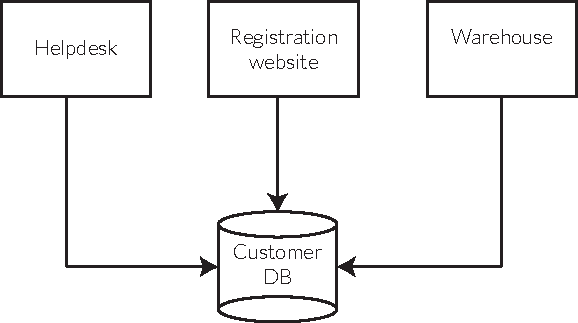
\includegraphics[scale=0.9]{figures/database_shared}
	\caption{The shared database}
	\label{fig:shared_database}
\end{figure}

\noindent This approach can introduce lots of difficulties. In this approach we allow different services to view and bind to the internal implementation details of the database schema. All services using this shared database have access and basically the database is shared in its entirety. If a service wants to change the schema of better represent the data, or make the service easier to maintain, all services using the database will break. Further this approach ties consumers of the database to a specific technology choice. As Sam Newman \cite[p. 41]{newman2015building} mentions, \textit{perhaps right now it makes sense to store customers in a relational database. But what if we over time realize we would be better off storing a a nonrelational database?}. This approach has high coupling between services that consumes the database and database itself, which is not desirable.

 \subsection*{One database per service}
 Instead of the \textit{shared database} approach, microservices architects favours the approach of splitting the monolithic database into separate databases that are only connected to one service. This approach tackles the problems mentioned with the shared database. The individual services hides the internal implementation details of the underlying database schema, and therefor we can change the underlying schema without necessarily breaking our consumers. Further we can choose the specific database system that will handle the task at hand in the most appropriate fashion. If a NoSQL database is the better choice, we choose this.\\
 
 \noindent Much research have been carried out into the topic of databases, and also in databases in distributed systems and also how to ensure resilience, with e.g. as replicasets in mongodb, a NoSQL database, that has features for replicating data across a cluster by assigning a primary database and syncing with the replicas. Another topic within this field is \textit{database sharding}, which is a horizontal partition of data. An example os a scenario where this could be relevant is if we are implementing a database at global scale, and we want to let users in e.g. America only communicate with the shard in America instead of a centralized database. However it is still possible as an administrator to collect data in unified manner across shards. This was a brief introduction to the role of databases in a microservice setup, this is not the scope of this present master thesis and will not be discussed further.